% Options for packages loaded elsewhere
\PassOptionsToPackage{unicode}{hyperref}
\PassOptionsToPackage{hyphens}{url}
%
\documentclass[
]{article}
\usepackage{amsmath,amssymb}
\usepackage{iftex}
\ifPDFTeX
  \usepackage[T1]{fontenc}
  \usepackage[utf8]{inputenc}
  \usepackage{textcomp} % provide euro and other symbols
\else % if luatex or xetex
  \usepackage{unicode-math} % this also loads fontspec
  \defaultfontfeatures{Scale=MatchLowercase}
  \defaultfontfeatures[\rmfamily]{Ligatures=TeX,Scale=1}
\fi
\usepackage{lmodern}
\ifPDFTeX\else
  % xetex/luatex font selection
\fi
% Use upquote if available, for straight quotes in verbatim environments
\IfFileExists{upquote.sty}{\usepackage{upquote}}{}
\IfFileExists{microtype.sty}{% use microtype if available
  \usepackage[]{microtype}
  \UseMicrotypeSet[protrusion]{basicmath} % disable protrusion for tt fonts
}{}
\makeatletter
\@ifundefined{KOMAClassName}{% if non-KOMA class
  \IfFileExists{parskip.sty}{%
    \usepackage{parskip}
  }{% else
    \setlength{\parindent}{0pt}
    \setlength{\parskip}{6pt plus 2pt minus 1pt}}
}{% if KOMA class
  \KOMAoptions{parskip=half}}
\makeatother
\usepackage{xcolor}
\usepackage[margin=1in]{geometry}
\usepackage{color}
\usepackage{fancyvrb}
\newcommand{\VerbBar}{|}
\newcommand{\VERB}{\Verb[commandchars=\\\{\}]}
\DefineVerbatimEnvironment{Highlighting}{Verbatim}{commandchars=\\\{\}}
% Add ',fontsize=\small' for more characters per line
\usepackage{framed}
\definecolor{shadecolor}{RGB}{248,248,248}
\newenvironment{Shaded}{\begin{snugshade}}{\end{snugshade}}
\newcommand{\AlertTok}[1]{\textcolor[rgb]{0.94,0.16,0.16}{#1}}
\newcommand{\AnnotationTok}[1]{\textcolor[rgb]{0.56,0.35,0.01}{\textbf{\textit{#1}}}}
\newcommand{\AttributeTok}[1]{\textcolor[rgb]{0.13,0.29,0.53}{#1}}
\newcommand{\BaseNTok}[1]{\textcolor[rgb]{0.00,0.00,0.81}{#1}}
\newcommand{\BuiltInTok}[1]{#1}
\newcommand{\CharTok}[1]{\textcolor[rgb]{0.31,0.60,0.02}{#1}}
\newcommand{\CommentTok}[1]{\textcolor[rgb]{0.56,0.35,0.01}{\textit{#1}}}
\newcommand{\CommentVarTok}[1]{\textcolor[rgb]{0.56,0.35,0.01}{\textbf{\textit{#1}}}}
\newcommand{\ConstantTok}[1]{\textcolor[rgb]{0.56,0.35,0.01}{#1}}
\newcommand{\ControlFlowTok}[1]{\textcolor[rgb]{0.13,0.29,0.53}{\textbf{#1}}}
\newcommand{\DataTypeTok}[1]{\textcolor[rgb]{0.13,0.29,0.53}{#1}}
\newcommand{\DecValTok}[1]{\textcolor[rgb]{0.00,0.00,0.81}{#1}}
\newcommand{\DocumentationTok}[1]{\textcolor[rgb]{0.56,0.35,0.01}{\textbf{\textit{#1}}}}
\newcommand{\ErrorTok}[1]{\textcolor[rgb]{0.64,0.00,0.00}{\textbf{#1}}}
\newcommand{\ExtensionTok}[1]{#1}
\newcommand{\FloatTok}[1]{\textcolor[rgb]{0.00,0.00,0.81}{#1}}
\newcommand{\FunctionTok}[1]{\textcolor[rgb]{0.13,0.29,0.53}{\textbf{#1}}}
\newcommand{\ImportTok}[1]{#1}
\newcommand{\InformationTok}[1]{\textcolor[rgb]{0.56,0.35,0.01}{\textbf{\textit{#1}}}}
\newcommand{\KeywordTok}[1]{\textcolor[rgb]{0.13,0.29,0.53}{\textbf{#1}}}
\newcommand{\NormalTok}[1]{#1}
\newcommand{\OperatorTok}[1]{\textcolor[rgb]{0.81,0.36,0.00}{\textbf{#1}}}
\newcommand{\OtherTok}[1]{\textcolor[rgb]{0.56,0.35,0.01}{#1}}
\newcommand{\PreprocessorTok}[1]{\textcolor[rgb]{0.56,0.35,0.01}{\textit{#1}}}
\newcommand{\RegionMarkerTok}[1]{#1}
\newcommand{\SpecialCharTok}[1]{\textcolor[rgb]{0.81,0.36,0.00}{\textbf{#1}}}
\newcommand{\SpecialStringTok}[1]{\textcolor[rgb]{0.31,0.60,0.02}{#1}}
\newcommand{\StringTok}[1]{\textcolor[rgb]{0.31,0.60,0.02}{#1}}
\newcommand{\VariableTok}[1]{\textcolor[rgb]{0.00,0.00,0.00}{#1}}
\newcommand{\VerbatimStringTok}[1]{\textcolor[rgb]{0.31,0.60,0.02}{#1}}
\newcommand{\WarningTok}[1]{\textcolor[rgb]{0.56,0.35,0.01}{\textbf{\textit{#1}}}}
\usepackage{graphicx}
\makeatletter
\def\maxwidth{\ifdim\Gin@nat@width>\linewidth\linewidth\else\Gin@nat@width\fi}
\def\maxheight{\ifdim\Gin@nat@height>\textheight\textheight\else\Gin@nat@height\fi}
\makeatother
% Scale images if necessary, so that they will not overflow the page
% margins by default, and it is still possible to overwrite the defaults
% using explicit options in \includegraphics[width, height, ...]{}
\setkeys{Gin}{width=\maxwidth,height=\maxheight,keepaspectratio}
% Set default figure placement to htbp
\makeatletter
\def\fps@figure{htbp}
\makeatother
\setlength{\emergencystretch}{3em} % prevent overfull lines
\providecommand{\tightlist}{%
  \setlength{\itemsep}{0pt}\setlength{\parskip}{0pt}}
\setcounter{secnumdepth}{-\maxdimen} % remove section numbering
\ifLuaTeX
  \usepackage{selnolig}  % disable illegal ligatures
\fi
\IfFileExists{bookmark.sty}{\usepackage{bookmark}}{\usepackage{hyperref}}
\IfFileExists{xurl.sty}{\usepackage{xurl}}{} % add URL line breaks if available
\urlstyle{same}
\hypersetup{
  pdftitle={Code-Along-And-Challenge-9},
  pdfauthor={Ariel Quek},
  hidelinks,
  pdfcreator={LaTeX via pandoc}}

\title{Code-Along-And-Challenge-9}
\author{Ariel Quek}
\date{2023-10-16}

\begin{document}
\maketitle

\begin{Shaded}
\begin{Highlighting}[]
\NormalTok{knitr}\SpecialCharTok{::}\NormalTok{opts\_chunk}\SpecialCharTok{$}\FunctionTok{set}\NormalTok{(}\AttributeTok{echo =} \ConstantTok{TRUE}\NormalTok{)}
\end{Highlighting}
\end{Shaded}

\hypertarget{code-along-9}{%
\subsection{Code Along 9}\label{code-along-9}}

Part ONE: About tidy vs non-tidy data

\#Tidy data

\begin{Shaded}
\begin{Highlighting}[]
\FunctionTok{install.packages}\NormalTok{(}\StringTok{"tidyverse"}\NormalTok{, }\AttributeTok{repos =} \StringTok{"http://cran.us.r{-}project.org"}\NormalTok{)}
\end{Highlighting}
\end{Shaded}

\begin{verbatim}
## Installing package into 'C:/Users/Ariel/AppData/Local/R/win-library/4.2'
## (as 'lib' is unspecified)
\end{verbatim}

\begin{verbatim}
## package 'tidyverse' successfully unpacked and MD5 sums checked
## 
## The downloaded binary packages are in
##  C:\Users\Ariel\AppData\Local\Temp\RtmpKkyyNT\downloaded_packages
\end{verbatim}

\begin{Shaded}
\begin{Highlighting}[]
\FunctionTok{library}\NormalTok{(tidyverse)}
\end{Highlighting}
\end{Shaded}

\begin{verbatim}
## Warning: package 'tidyverse' was built under R version 4.2.3
\end{verbatim}

\begin{verbatim}
## Warning: package 'ggplot2' was built under R version 4.2.3
\end{verbatim}

\begin{verbatim}
## Warning: package 'tibble' was built under R version 4.2.1
\end{verbatim}

\begin{verbatim}
## Warning: package 'tidyr' was built under R version 4.2.2
\end{verbatim}

\begin{verbatim}
## Warning: package 'readr' was built under R version 4.2.3
\end{verbatim}

\begin{verbatim}
## Warning: package 'purrr' was built under R version 4.2.2
\end{verbatim}

\begin{verbatim}
## Warning: package 'dplyr' was built under R version 4.2.2
\end{verbatim}

\begin{verbatim}
## Warning: package 'stringr' was built under R version 4.2.2
\end{verbatim}

\begin{verbatim}
## Warning: package 'forcats' was built under R version 4.2.3
\end{verbatim}

\begin{verbatim}
## Warning: package 'lubridate' was built under R version 4.2.3
\end{verbatim}

\begin{verbatim}
## -- Attaching core tidyverse packages ------------------------ tidyverse 2.0.0 --
## v dplyr     1.1.0     v readr     2.1.4
## v forcats   1.0.0     v stringr   1.5.0
## v ggplot2   3.4.3     v tibble    3.1.8
## v lubridate 1.9.2     v tidyr     1.3.0
## v purrr     1.0.1
\end{verbatim}

\begin{verbatim}
## -- Conflicts ------------------------------------------ tidyverse_conflicts() --
## x dplyr::filter() masks stats::filter()
## x dplyr::lag()    masks stats::lag()
## i Use the ]8;;http://conflicted.r-lib.org/conflicted package]8;; to force all conflicts to become errors
\end{verbatim}

\begin{Shaded}
\begin{Highlighting}[]
\NormalTok{tidydata }\OtherTok{\textless{}{-}} \FunctionTok{tribble}\NormalTok{( }\SpecialCharTok{\textasciitilde{}}\NormalTok{country, }\SpecialCharTok{\textasciitilde{}}\NormalTok{year, }\SpecialCharTok{\textasciitilde{}}\NormalTok{cases, }\SpecialCharTok{\textasciitilde{}}\NormalTok{population, }\StringTok{"Afghanistan"}\NormalTok{, }\DecValTok{1999}\NormalTok{, }\DecValTok{745}\NormalTok{, }\DecValTok{19987071}\NormalTok{,}
\StringTok{"Afghanistan"}\NormalTok{, }\DecValTok{2000}\NormalTok{, }\DecValTok{2666}\NormalTok{, }\DecValTok{20595360}\NormalTok{,}
\StringTok{"Brazil"}\NormalTok{, }\DecValTok{1999}\NormalTok{, }\DecValTok{37737}\NormalTok{, }\DecValTok{172006362}\NormalTok{,}
\StringTok{"Brazil"}\NormalTok{, }\DecValTok{2000}\NormalTok{, }\DecValTok{80488}\NormalTok{, }\DecValTok{174504898}\NormalTok{,}
\StringTok{"China"}\NormalTok{, }\DecValTok{1999}\NormalTok{, }\DecValTok{212258}\NormalTok{, }\DecValTok{1272915272}\NormalTok{,}
\StringTok{"China"}\NormalTok{, }\DecValTok{2000}\NormalTok{, }\DecValTok{213766}\NormalTok{, }\DecValTok{1280428583}\NormalTok{)}

\NormalTok{tidydata}
\end{Highlighting}
\end{Shaded}

\begin{verbatim}
## # A tibble: 6 x 4
##   country      year  cases population
##   <chr>       <dbl>  <dbl>      <dbl>
## 1 Afghanistan  1999    745   19987071
## 2 Afghanistan  2000   2666   20595360
## 3 Brazil       1999  37737  172006362
## 4 Brazil       2000  80488  174504898
## 5 China        1999 212258 1272915272
## 6 China        2000 213766 1280428583
\end{verbatim}

\#Non-tidy data

\begin{verbatim}
## # A tibble: 6 x 3
##   country      year rate             
##   <chr>       <dbl> <chr>            
## 1 Afghanistan  1999 745/19987071     
## 2 Afghanistan  2000 2666/20595360    
## 3 Brazil       1999 37737/172006362  
## 4 Brazil       2000 80488/174504898  
## 5 China        1999 212258/1272915272
## 6 China        2000 213766/1280428583
\end{verbatim}

\#Example of benefit of tidy data (slide 9)

\begin{Shaded}
\begin{Highlighting}[]
\NormalTok{tidydata }\SpecialCharTok{\%\textgreater{}\%}
 \FunctionTok{group\_by}\NormalTok{(year) }\SpecialCharTok{\%\textgreater{}\%}
 \FunctionTok{summarize}\NormalTok{(}\AttributeTok{total\_cases =} \FunctionTok{sum}\NormalTok{(cases))}
\end{Highlighting}
\end{Shaded}

\begin{verbatim}
## # A tibble: 2 x 2
##    year total_cases
##   <dbl>       <dbl>
## 1  1999      250740
## 2  2000      296920
\end{verbatim}

\#How to tidy data - Example 1 (slides 11-13)

\begin{Shaded}
\begin{Highlighting}[]
\NormalTok{tidieddata }\OtherTok{\textless{}{-}}\NormalTok{ nontidydata }\SpecialCharTok{\%\textgreater{}\%}
 \FunctionTok{separate}\NormalTok{(rate, }\AttributeTok{into =} \FunctionTok{c}\NormalTok{(}\StringTok{"cases"}\NormalTok{,}
 \StringTok{"population"}\NormalTok{),}
 \AttributeTok{sep =} \StringTok{"/"}\NormalTok{)}

\NormalTok{tidieddata}
\end{Highlighting}
\end{Shaded}

\begin{verbatim}
## # A tibble: 6 x 4
##   country      year cases  population
##   <chr>       <dbl> <chr>  <chr>     
## 1 Afghanistan  1999 745    19987071  
## 2 Afghanistan  2000 2666   20595360  
## 3 Brazil       1999 37737  172006362 
## 4 Brazil       2000 80488  174504898 
## 5 China        1999 212258 1272915272
## 6 China        2000 213766 1280428583
\end{verbatim}

\begin{Shaded}
\begin{Highlighting}[]
\NormalTok{newtidieddata }\OtherTok{\textless{}{-}}\NormalTok{ tidieddata }\SpecialCharTok{\%\textgreater{}\%}
 \FunctionTok{pivot\_longer}\NormalTok{(}
 \AttributeTok{cols =}\NormalTok{ cases}\SpecialCharTok{:}\NormalTok{population,}
 \AttributeTok{names\_to =} \StringTok{"measurement"}
\NormalTok{,}
 \AttributeTok{values\_to =} \StringTok{"value"}
\NormalTok{ )}

\NormalTok{newtidieddata}
\end{Highlighting}
\end{Shaded}

\begin{verbatim}
## # A tibble: 12 x 4
##    country      year measurement value     
##    <chr>       <dbl> <chr>       <chr>     
##  1 Afghanistan  1999 cases       745       
##  2 Afghanistan  1999 population  19987071  
##  3 Afghanistan  2000 cases       2666      
##  4 Afghanistan  2000 population  20595360  
##  5 Brazil       1999 cases       37737     
##  6 Brazil       1999 population  172006362 
##  7 Brazil       2000 cases       80488     
##  8 Brazil       2000 population  174504898 
##  9 China        1999 cases       212258    
## 10 China        1999 population  1272915272
## 11 China        2000 cases       213766    
## 12 China        2000 population  1280428583
\end{verbatim}

\begin{Shaded}
\begin{Highlighting}[]
\FunctionTok{ggplot}\NormalTok{(newtidieddata) }\SpecialCharTok{+}
 \FunctionTok{aes}\NormalTok{(}\AttributeTok{x=}\NormalTok{year,}\AttributeTok{y=}\NormalTok{value, }\AttributeTok{colour=}\NormalTok{country) }\SpecialCharTok{+}
 \FunctionTok{geom\_point}\NormalTok{() }\SpecialCharTok{+}
 \FunctionTok{geom\_line}\NormalTok{(}\FunctionTok{aes}\NormalTok{(}\AttributeTok{group =}\NormalTok{ country))}\SpecialCharTok{+}
 \FunctionTok{facet\_wrap}\NormalTok{(}\SpecialCharTok{\textasciitilde{}}\NormalTok{measurement) }\SpecialCharTok{+}
 \FunctionTok{theme\_bw}\NormalTok{()}
\end{Highlighting}
\end{Shaded}

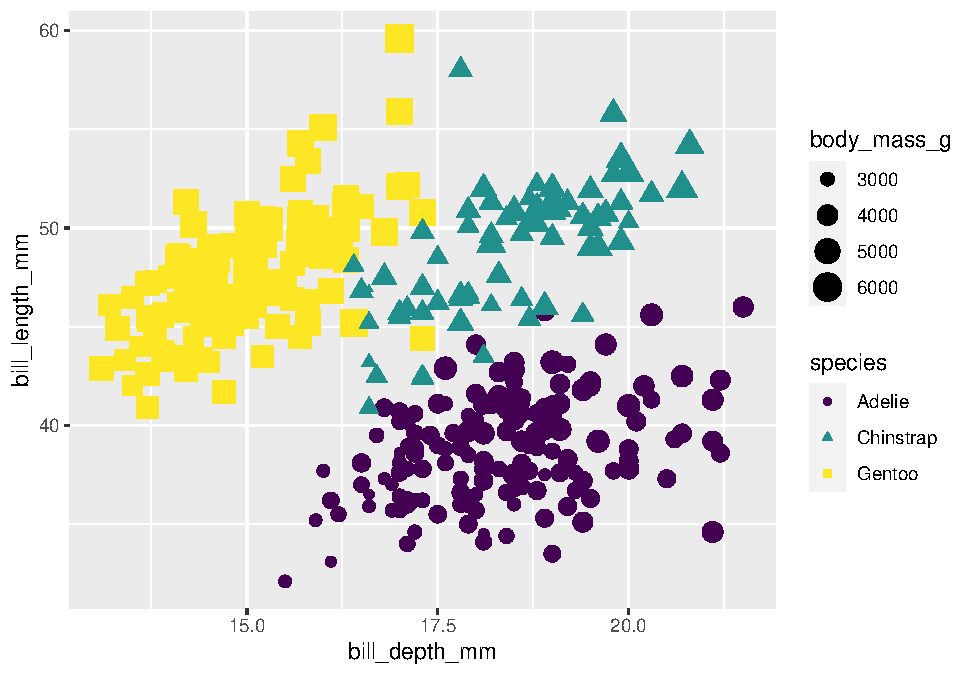
\includegraphics{Code-Along-And-Challenge-9_files/figure-latex/unnamed-chunk-4-1.pdf}

\#How to reshape data using ``pivot\_longer'' - Example 2 (slides 14-17)

\begin{Shaded}
\begin{Highlighting}[]
\NormalTok{df }\OtherTok{\textless{}{-}} \FunctionTok{tribble}\NormalTok{(}
 \SpecialCharTok{\textasciitilde{}}\NormalTok{id, }\SpecialCharTok{\textasciitilde{}}\NormalTok{bp1, }\SpecialCharTok{\textasciitilde{}}\NormalTok{bp2,}
 \StringTok{"A"}\NormalTok{, }\DecValTok{100}\NormalTok{, }\DecValTok{120}\NormalTok{,}
 \StringTok{"B"}\NormalTok{, }\DecValTok{140}\NormalTok{, }\DecValTok{115}\NormalTok{,}
 \StringTok{"C"}\NormalTok{, }\DecValTok{120}\NormalTok{, }\DecValTok{125}\NormalTok{)}

\NormalTok{df}
\end{Highlighting}
\end{Shaded}

\begin{verbatim}
## # A tibble: 3 x 3
##   id      bp1   bp2
##   <chr> <dbl> <dbl>
## 1 A       100   120
## 2 B       140   115
## 3 C       120   125
\end{verbatim}

\begin{Shaded}
\begin{Highlighting}[]
\NormalTok{df }\SpecialCharTok{\%\textgreater{}\%}
 \FunctionTok{pivot\_longer}\NormalTok{(}
 \AttributeTok{cols =}\NormalTok{ bp1}\SpecialCharTok{:}\NormalTok{bp2,}
 \AttributeTok{names\_to =} \StringTok{"measurement"}\NormalTok{,}
 \AttributeTok{values\_to =} \StringTok{"value"}
\NormalTok{ )}
\end{Highlighting}
\end{Shaded}

\begin{verbatim}
## # A tibble: 6 x 3
##   id    measurement value
##   <chr> <chr>       <dbl>
## 1 A     bp1           100
## 2 A     bp2           120
## 3 B     bp1           140
## 4 B     bp2           115
## 5 C     bp1           120
## 6 C     bp2           125
\end{verbatim}

\#How to reshape data using ``pivot\_wider'' - Example 3 (slide 18)

\begin{Shaded}
\begin{Highlighting}[]
\NormalTok{newtidieddata}
\end{Highlighting}
\end{Shaded}

\begin{verbatim}
## # A tibble: 12 x 4
##    country      year measurement value     
##    <chr>       <dbl> <chr>       <chr>     
##  1 Afghanistan  1999 cases       745       
##  2 Afghanistan  1999 population  19987071  
##  3 Afghanistan  2000 cases       2666      
##  4 Afghanistan  2000 population  20595360  
##  5 Brazil       1999 cases       37737     
##  6 Brazil       1999 population  172006362 
##  7 Brazil       2000 cases       80488     
##  8 Brazil       2000 population  174504898 
##  9 China        1999 cases       212258    
## 10 China        1999 population  1272915272
## 11 China        2000 cases       213766    
## 12 China        2000 population  1280428583
\end{verbatim}

\begin{Shaded}
\begin{Highlighting}[]
\NormalTok{newtidieddata }\SpecialCharTok{\%\textgreater{}\%} \FunctionTok{pivot\_wider}\NormalTok{(}\AttributeTok{names\_from=}\StringTok{"measurement"}\NormalTok{, }
                              \AttributeTok{values\_from =}\StringTok{"value"}\NormalTok{)}
\end{Highlighting}
\end{Shaded}

\begin{verbatim}
## # A tibble: 6 x 4
##   country      year cases  population
##   <chr>       <dbl> <chr>  <chr>     
## 1 Afghanistan  1999 745    19987071  
## 2 Afghanistan  2000 2666   20595360  
## 3 Brazil       1999 37737  172006362 
## 4 Brazil       2000 80488  174504898 
## 5 China        1999 212258 1272915272
## 6 China        2000 213766 1280428583
\end{verbatim}

\#Reshaping data using ``pivot\_wider'' - Example 4 (slide 19)

\begin{Shaded}
\begin{Highlighting}[]
\NormalTok{df }\OtherTok{\textless{}{-}} \FunctionTok{tribble}\NormalTok{(}
 \SpecialCharTok{\textasciitilde{}}\NormalTok{id, }\SpecialCharTok{\textasciitilde{}}\NormalTok{measurement, }\SpecialCharTok{\textasciitilde{}}\NormalTok{value,}
 \StringTok{"A"}\NormalTok{, }\StringTok{"bp1"}\NormalTok{, }\DecValTok{100}\NormalTok{,}
 \StringTok{"B"}\NormalTok{, }\StringTok{"bp1"}\NormalTok{, }\DecValTok{140}\NormalTok{,}
 \StringTok{"B"}\NormalTok{, }\StringTok{"bp2"}\NormalTok{, }\DecValTok{115}\NormalTok{,}
 \StringTok{"A"}\NormalTok{, }\StringTok{"bp2"}\NormalTok{, }\DecValTok{120}\NormalTok{,}
 \StringTok{"A"}\NormalTok{, }\StringTok{"bp3"}\NormalTok{, }\DecValTok{105}\NormalTok{)}
\NormalTok{df}
\end{Highlighting}
\end{Shaded}

\begin{verbatim}
## # A tibble: 5 x 3
##   id    measurement value
##   <chr> <chr>       <dbl>
## 1 A     bp1           100
## 2 B     bp1           140
## 3 B     bp2           115
## 4 A     bp2           120
## 5 A     bp3           105
\end{verbatim}

\begin{Shaded}
\begin{Highlighting}[]
\NormalTok{df }\SpecialCharTok{\%\textgreater{}\%}
 \FunctionTok{pivot\_wider}\NormalTok{(}
 \AttributeTok{names\_from =}\NormalTok{ measurement,}
 \AttributeTok{values\_from =}\NormalTok{ value)}
\end{Highlighting}
\end{Shaded}

\begin{verbatim}
## # A tibble: 2 x 4
##   id      bp1   bp2   bp3
##   <chr> <dbl> <dbl> <dbl>
## 1 A       100   120   105
## 2 B       140   115    NA
\end{verbatim}

\hypertarget{challenge-9}{%
\subsection{Challenge 9}\label{challenge-9}}

\hypertarget{question-1}{%
\section{Question 1}\label{question-1}}

\begin{Shaded}
\begin{Highlighting}[]
\FunctionTok{library}\NormalTok{(tidyverse)}
\NormalTok{billboard}
\end{Highlighting}
\end{Shaded}

\begin{verbatim}
## # A tibble: 317 x 79
##    artist     track date.entered   wk1   wk2   wk3   wk4   wk5   wk6   wk7   wk8
##    <chr>      <chr> <date>       <dbl> <dbl> <dbl> <dbl> <dbl> <dbl> <dbl> <dbl>
##  1 2 Pac      Baby~ 2000-02-26      87    82    72    77    87    94    99    NA
##  2 2Ge+her    The ~ 2000-09-02      91    87    92    NA    NA    NA    NA    NA
##  3 3 Doors D~ Kryp~ 2000-04-08      81    70    68    67    66    57    54    53
##  4 3 Doors D~ Loser 2000-10-21      76    76    72    69    67    65    55    59
##  5 504 Boyz   Wobb~ 2000-04-15      57    34    25    17    17    31    36    49
##  6 98^0       Give~ 2000-08-19      51    39    34    26    26    19     2     2
##  7 A*Teens    Danc~ 2000-07-08      97    97    96    95   100    NA    NA    NA
##  8 Aaliyah    I Do~ 2000-01-29      84    62    51    41    38    35    35    38
##  9 Aaliyah    Try ~ 2000-03-18      59    53    38    28    21    18    16    14
## 10 Adams, Yo~ Open~ 2000-08-26      76    76    74    69    68    67    61    58
## # i 307 more rows
## # i 68 more variables: wk9 <dbl>, wk10 <dbl>, wk11 <dbl>, wk12 <dbl>,
## #   wk13 <dbl>, wk14 <dbl>, wk15 <dbl>, wk16 <dbl>, wk17 <dbl>, wk18 <dbl>,
## #   wk19 <dbl>, wk20 <dbl>, wk21 <dbl>, wk22 <dbl>, wk23 <dbl>, wk24 <dbl>,
## #   wk25 <dbl>, wk26 <dbl>, wk27 <dbl>, wk28 <dbl>, wk29 <dbl>, wk30 <dbl>,
## #   wk31 <dbl>, wk32 <dbl>, wk33 <dbl>, wk34 <dbl>, wk35 <dbl>, wk36 <dbl>,
## #   wk37 <dbl>, wk38 <dbl>, wk39 <dbl>, wk40 <dbl>, wk41 <dbl>, wk42 <dbl>, ...
\end{verbatim}

\begin{Shaded}
\begin{Highlighting}[]
\NormalTok{billboard\_new }\OtherTok{\textless{}{-}}\NormalTok{ billboard }\SpecialCharTok{\%\textgreater{}\%} 
  \FunctionTok{pivot\_longer}\NormalTok{(}
    \AttributeTok{cols=}\FunctionTok{starts\_with}\NormalTok{(}\StringTok{"wk"}\NormalTok{),}
    \AttributeTok{names\_to=}\StringTok{"week"}\NormalTok{,}
    \AttributeTok{values\_to=}\StringTok{"value"}\NormalTok{,}
    \AttributeTok{values\_drop\_na =} \ConstantTok{TRUE}\NormalTok{) }\SpecialCharTok{\%\textgreater{}\%} \FunctionTok{mutate}\NormalTok{(}\AttributeTok{week =} \FunctionTok{parse\_number}\NormalTok{(week))}
\NormalTok{billboard\_new}
\end{Highlighting}
\end{Shaded}

\begin{verbatim}
## # A tibble: 5,307 x 5
##    artist  track                   date.entered  week value
##    <chr>   <chr>                   <date>       <dbl> <dbl>
##  1 2 Pac   Baby Don't Cry (Keep... 2000-02-26       1    87
##  2 2 Pac   Baby Don't Cry (Keep... 2000-02-26       2    82
##  3 2 Pac   Baby Don't Cry (Keep... 2000-02-26       3    72
##  4 2 Pac   Baby Don't Cry (Keep... 2000-02-26       4    77
##  5 2 Pac   Baby Don't Cry (Keep... 2000-02-26       5    87
##  6 2 Pac   Baby Don't Cry (Keep... 2000-02-26       6    94
##  7 2 Pac   Baby Don't Cry (Keep... 2000-02-26       7    99
##  8 2Ge+her The Hardest Part Of ... 2000-09-02       1    91
##  9 2Ge+her The Hardest Part Of ... 2000-09-02       2    87
## 10 2Ge+her The Hardest Part Of ... 2000-09-02       3    92
## # i 5,297 more rows
\end{verbatim}

\begin{Shaded}
\begin{Highlighting}[]
\FunctionTok{library}\NormalTok{(ggplot2)}
\CommentTok{\# Creating a plot of rankings of tracks across time}
\FunctionTok{ggplot}\NormalTok{(}\AttributeTok{data=}\NormalTok{billboard\_new, }
       \AttributeTok{mapping =} \FunctionTok{aes}\NormalTok{(}\AttributeTok{x =}\NormalTok{ week,}
                     \AttributeTok{y =}\NormalTok{ value)) }\SpecialCharTok{+} 
         \FunctionTok{geom\_line}\NormalTok{(}\AttributeTok{color=}\StringTok{"purple"}\NormalTok{) }\SpecialCharTok{+}
         \FunctionTok{labs}\NormalTok{(}\AttributeTok{title =} \StringTok{"Rank of tracks across time"}\NormalTok{,}
              \AttributeTok{x =}\StringTok{"Week"}\NormalTok{, }
              \AttributeTok{y =} \StringTok{"Rank"}\NormalTok{)}
\end{Highlighting}
\end{Shaded}

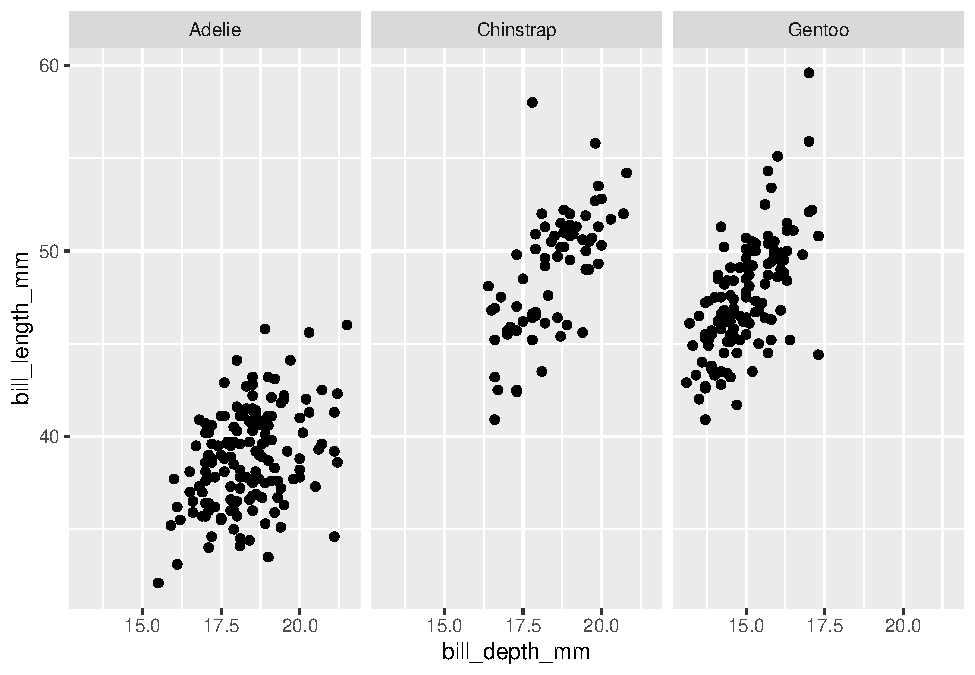
\includegraphics{Code-Along-And-Challenge-9_files/figure-latex/unnamed-chunk-9-1.pdf}

\hypertarget{question-2}{%
\section{Question 2}\label{question-2}}

\begin{Shaded}
\begin{Highlighting}[]
\NormalTok{cms\_patient\_experience}
\end{Highlighting}
\end{Shaded}

\begin{verbatim}
## # A tibble: 500 x 5
##    org_pac_id org_nm                           measure_cd measure_title prf_rate
##    <chr>      <chr>                            <chr>      <chr>            <dbl>
##  1 0446157747 USC CARE MEDICAL GROUP INC       CAHPS_GRP~ CAHPS for MI~       63
##  2 0446157747 USC CARE MEDICAL GROUP INC       CAHPS_GRP~ CAHPS for MI~       87
##  3 0446157747 USC CARE MEDICAL GROUP INC       CAHPS_GRP~ CAHPS for MI~       86
##  4 0446157747 USC CARE MEDICAL GROUP INC       CAHPS_GRP~ CAHPS for MI~       57
##  5 0446157747 USC CARE MEDICAL GROUP INC       CAHPS_GRP~ CAHPS for MI~       85
##  6 0446157747 USC CARE MEDICAL GROUP INC       CAHPS_GRP~ CAHPS for MI~       24
##  7 0446162697 ASSOCIATION OF UNIVERSITY PHYSI~ CAHPS_GRP~ CAHPS for MI~       59
##  8 0446162697 ASSOCIATION OF UNIVERSITY PHYSI~ CAHPS_GRP~ CAHPS for MI~       85
##  9 0446162697 ASSOCIATION OF UNIVERSITY PHYSI~ CAHPS_GRP~ CAHPS for MI~       83
## 10 0446162697 ASSOCIATION OF UNIVERSITY PHYSI~ CAHPS_GRP~ CAHPS for MI~       63
## # i 490 more rows
\end{verbatim}

\begin{Shaded}
\begin{Highlighting}[]
\DocumentationTok{\#\# A data set that collects data about patient experiences }
\NormalTok{patients }\OtherTok{\textless{}{-}}\NormalTok{ cms\_patient\_experience }\SpecialCharTok{\%\textgreater{}\%}
  \FunctionTok{pivot\_wider}\NormalTok{(}\AttributeTok{names\_from =}\NormalTok{ measure\_cd, }
              \AttributeTok{values\_from=}\NormalTok{ prf\_rate,}
              \AttributeTok{id\_cols=}\FunctionTok{starts\_with}\NormalTok{(}\StringTok{"org"}\NormalTok{))}

\DocumentationTok{\#\#to get unique IDs}
\NormalTok{uniqueIDs }\OtherTok{\textless{}{-}}\NormalTok{ patients }\SpecialCharTok{\%\textgreater{}\%} 
  \FunctionTok{select}\NormalTok{(org\_pac\_id,org\_nm) }\SpecialCharTok{\%\textgreater{}\%} 
  \FunctionTok{distinct}\NormalTok{()}
\NormalTok{uniqueIDs}
\end{Highlighting}
\end{Shaded}

\begin{verbatim}
## # A tibble: 95 x 2
##    org_pac_id org_nm                                    
##    <chr>      <chr>                                     
##  1 0446157747 USC CARE MEDICAL GROUP INC                
##  2 0446162697 ASSOCIATION OF UNIVERSITY PHYSICIANS      
##  3 0547164295 BEAVER MEDICAL GROUP PC                   
##  4 0749333730 CAPE PHYSICIANS ASSOCIATES PA             
##  5 0840104360 ALLIANCE PHYSICIANS INC                   
##  6 0840109864 REX HOSPITAL INC                          
##  7 0840513552 SCL HEALTH MEDICAL GROUP DENVER LLC       
##  8 0941545784 GRITMAN MEDICAL CENTER INC                
##  9 1052612785 COMMUNITY MEDICAL GROUP LLC               
## 10 1254237779 OUR LADY OF LOURDES MEMORIAL HOSPITAL, INC
## # i 85 more rows
\end{verbatim}

Thank You!

\end{document}
